\documentclass[journal]{IEEEtran}
\usepackage[brazil]{babel}
\usepackage[utf8]{inputenc}
\usepackage[pdftex]{graphicx}

\begin{document}
	
%Titulo do artigo
\title{Controle e supervisão de um sistema de caldeira simulado}

%Nomes dos autores
\author{Autor 1~Autor 2~Autor 3% <-this % stops a space
\thanks{A. 1, Universidade Federal do Ceará, Sobral, Brasil e-mail: autor1@sobral.ufc.br.}% <-this % stops a space
\thanks{A. 2, Universidade Federal do Ceará, Sobral, Brasil, e-mail: autor2@sobral.ufc.br.}% <-this % stops a space
\thanks{A. 3, Universidade Federal do Ceará, Sobral, Brasil, e-mail: autor3@sobral.ufc.br.}% <-this % stops a space
}

% The paper headers
\markboth{SBL0092 - SOFTWARE EM TEMPO REAL}%
{Shell \MakeLowercase{\textit{et al.}}: Bare Demo of IEEEtran.cls for IEEE Journals}


% make the title area
\maketitle

% As a general rule, do not put math, special symbols or citations
% in the abstract or keywords.
\begin{abstract}
Escreva um breve resumo sobre o trabalho...
\end{abstract}

% Note that keywords are not normally used for peerreview papers.
\begin{IEEEkeywords}
defina algumas palavras-chave para o trabalho separados por vírgula.
\end{IEEEkeywords}

\IEEEpeerreviewmaketitle

\section{Introdução}

\IEEEPARstart{E}{screva} uma breve introdução sobre os sistemas de tempo real, falando sobre o uso de mutex, monitores e por fim apresentando o que o trabalho pretende mostrar.

A idéia do monitor é tornar determinados recursos privativo as tarefas \cite{IEEEhowto:romulo}.
\section{Metodologia}

Apresente como o trabalho foi realizado, falando da Parte I e II da descrição. 

Use diagrama de blocos se possível para indicar as etapas realizadas no trabalho.

\section{Resultados e discussões}

Apresente os resultados da parte I e II e discuta os resultados de acordo com o que foi pedido. Veja o exemplo de como colocar imagens no artigo. A Figura \ref{fig1} ...

	\begin{figure}[h]
	\centering
	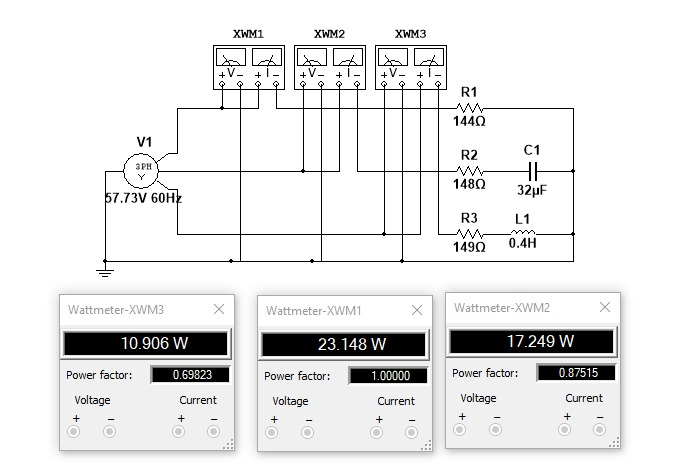
\includegraphics[width=3.5in]{Imagens/medidas.png}	
	\caption{Gráfico com as medições realizadas, na ordem dos casos de teste.}
	\label{fig1}
\end{figure}

%%%%%%%%%%%%%%%%%%%%%%%%%%%%%%%%%%%%%%%%%%%%%%%%5
%%%%%%%%%%%%%%%%%%%%%%%%%%%%%%%%%%%%%%%%%%%

\ifCLASSOPTIONcaptionsoff
  \newpage
\fi

\begin{thebibliography}{1}

\bibitem{IEEEhowto:romulo}
Oliveira, R. S. Fundamentos dos Sistemas de Tempo Real. Original registrado na Biblioteca Nacional. Primeira edição, revisão 3, outubro de 2018. ISBN-13: 9781728694047.

\end{thebibliography}

%%%%%%%%%%%%%%%%%%%%%%%%%%%%%%%%%%%%%%%%%
%Se tiver foto use essa forma
\begin{IEEEbiography}[{\includegraphics[width=1in,height=1.25in,clip,keepaspectratio]{Imagens/autor1.png}}]{Autor 1}
Texto da biografia aqui...
\end{IEEEbiography}

% Se não tem foto use essa forma
\begin{IEEEbiographynophoto}{Autor 2}
Texto da biografia aqui...
\end{IEEEbiographynophoto}


\begin{IEEEbiographynophoto}{Autor 3}
Texto da biografia aqui...
\end{IEEEbiographynophoto}


\end{document}